\section{Improper Integrals}\label{sec:ImproperIntegrals}
%%%%%%%%%%%%%%%%%%%%%%%%%%%%%%%%%%%%%%%%%%%%%%%%%%%
%Recall that the Fundamental Theorem of Calculus says that if $f$ is a \underline{{\bf continuous}} function on the closed interval $[a,b]$, then
%$$\ds{\int_a^b f(x)~dx=F(x)\bigg|_a^b=F(b)-F(a)},$$
%where $F$ is any antiderivative of $f$. 
%
%Both the {\bf continuity} condition and {\bf closed interval} must hold to use the Fundamental Theorem of Calculus, and in this case, $\ds\int_a^b f(x)\,dx$ represents the net area under $f(x)$ from $a$ to $b$: 
%$$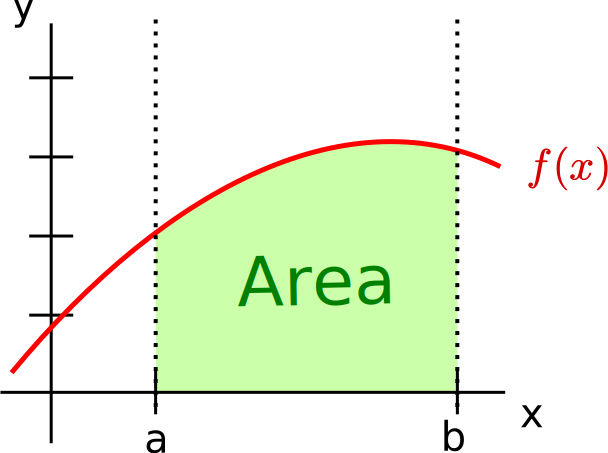
\includegraphics[width=2.25in]{images2/area-under}$$
%
%We begin with an example where blindly applying the Fundamental Theorem of Calculus can give an incorrect result.
%
%\begin{example}{Using FTC}{Using FTC}
%Explain why $\ds\int_{-1}^1\frac{1}{x^2}\,dx$ is not equal to $-2$.
%\end{example}  
%
%\begin{solution}
%Here is how one might proceed:  
%$$
%\int_{-1}^1\frac{1}{x^2}\,dx 
%~=~ \int_{-1}^1 x^{-2}\,dx 
%~=~ -x^{-1}\bigg|_{-1}^1 
%~=~ -\frac{1}{x}\bigg|_{-1}^1 
%~=~ \left(-\frac{1}{1}\right) - \left(-\frac{1}{(-1)}\right) 
%~=~ -2$$  
% However, the above answer is {\bf WRONG!} 
% Since $f(x)=1/x^2$ is not continuous on $[-1,~1]$, we cannot directly apply the Fundamental Theorem of Calculus.
%Intuitively, we can see why $-2$ is not the correct answer by looking at the graph of $f(x)=1/x^2$ on $[-1,~1]$.
%The shaded area appears to grow without bound as seen in the figure below.
%$$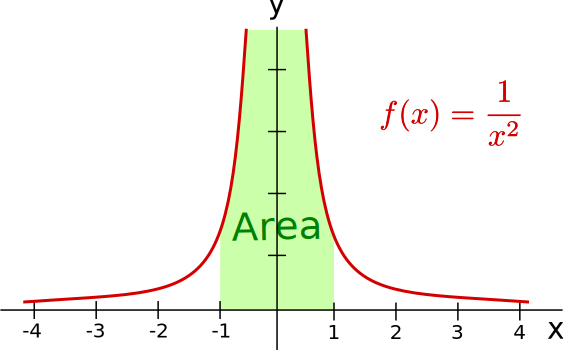
\includegraphics[width=2.5in]{images2/improper-integral-example-1}$$
%\end{solution}
%
%Formalizing this example leads to the concept of an improper integral.
%There are two ways to extend the Fundamental Theorem of Calculus.
%One is to use an {\bf infinite interval}, i.e., $[a,\infty)$, $(-\infty,b]$ or $(-\infty,\infty)$.
%The second is to allow the interval $[a,b]$ to contain an infinite {\bf discontinuity} of $f(x)$.
%In either case, the integral is called an {\bf improper integral}.  
%One of the most important applications of this concept is probability distributions.  
%
%To compute improper integrals, we use the concept of limits along with the Fundamental Theorem of Calculus.
% 
%\begin{definition}{Definitions for Improper Integrals}{Definitions for Improper Integrals}
%If $f(x)$ is continuous on $[a,\infty)$, then the improper integral of $f$ over $[a,\infty)$ is:
%$$\int_{a}^{\infty} f(x)\,dx:=\lim_{R\to\infty}\int_a^R f(x)\,dx.$$ 
%If $f(x)$ is continuous on $(-\infty,b]$, then the improper integral of $f$ over $(-\infty,b]$ is:
%$$\int_{-\infty}^b f(x)\,dx:=\lim_{R\to -\infty}\int_R^b f(x)\,dx.$$
%\end{definition}
%
%If the limit exists and is a finite number, we say the improper integral {\bf converges}. Otherwise, we say the  improper integral {\bf diverges}.
%
%To get an intuitive (though not completely correct) interpretation of improper integrals, we attempt to analyze $\ds\int_a^\infty f(x)\,dx$ graphically. 
% Here assume $f(x)$ is continuous on $[a,\infty)$: 
%$$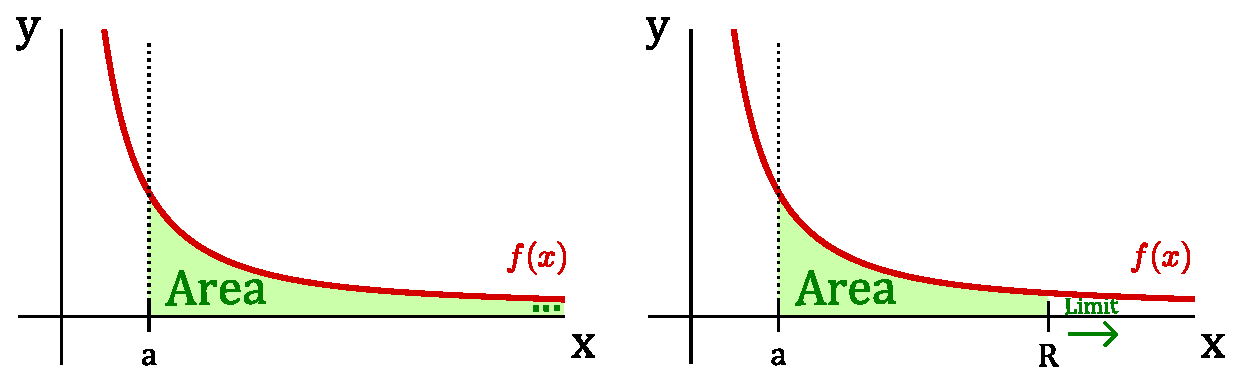
\includegraphics[width=5in]{images2/improper-integral-theory-2}$$ 
% We let $R$ be a fixed number in $[a,\infty)$. 
% Then by taking the limit as $R$ approaches $\infty$, we get the improper integral:  
%$$\int_a^\infty f(x)\,dx:=\lim_{R\to\infty}\int_a^R f(x)\,dx.$$ 
% We can then apply the Fundamental Theorem of Calculus to the last integral as $f(x)$ is continuous on the closed interval $[a,R]$.
%
%We next define the improper integral for the interval $(-\infty,~\infty)$.
%
%\begin{definition}{Definitions for Improper Integrals}{Definitions for Improper Integrals}
% If both $\ds\int_{-\infty}^a f(x)\,dx$ and $\ds\int_{a}^{\infty} f(x)\,dx$ are convergent, then the improper integral of $f$ over $(-\infty,\infty)$ is:
%$$\int_{-\infty}^{\infty} f(x)\,dx:=\int_{-\infty}^a f(x)\,dx+\int_{a}^{\infty} f(x)\,dx$$
%\end{definition}
%
%The above definition requires {\bf both} of the integrals
%$$\int_{-\infty}^a f(x)\,dx\qquad\mbox{and}\qquad\int_{a}^{\infty} f(x)\,dx$$
%to be convergent for $\ds\int_{-\infty}^{\infty} f(x)\,dx$ to also be convergent. 
% If {\bf either} of $\ds\int_{-\infty}^a f(x)\,dx$ or $\ds\int_{a}^{\infty} f(x)\,dx$ is divergent, then so is $\ds\int_{-\infty}^{\infty} f(x)\,dx$.
%
%\begin{example}{Improper Integral}{Improper Integral}
%Determine whether $\ds\int_1^\infty\frac{1}{x}\,dx$ is convergent or divergent.
%\end{example} 
%
%\begin{solution}
% Using the definition for improper integrals we write this as:
%$$	\int_1^\infty \frac{1}{x}\,dx= \lim_{R\to\infty} \int_1^R\frac{1}{x}\,dx
%	= \lim_{R\to\infty} \ln|x|\bigg|_1^R
%	=\lim_{R\to\infty} \ln|R| - \ln|1|
%	= \lim_{R\to\infty} \ln|R|
%	= +\infty$$
% Therefore, the integral is {\bf divergent}.
%\end{solution}
%
%\begin{example}{Improper Integral}{Improper Integral}
%Determine whether $\ds\int_{-\infty}^\infty x\sin(x^2)\,dx$ is convergent or divergent.
%\end{example}  
%
%\begin{solution}
% We must compute both $\ds\int_0^\infty x\sin(x^2)\,dx$ and $\ds\int_{-\infty}^0 x\sin(x^2)\,dx$.  
% Note that we don't have to split the integral up at $0$, any finite value $a$ will work.  
% First we compute the indefinite integral.  
% Let $u=x^2$, then $du=2x\,dx$ and hence, 
%$$\int x\sin(x^2)\,dx=\frac{1}{2} \int \sin(u)\,du=-\frac{1}{2}\cos(x^2)+C$$
%Using the definition of improper integral gives: 
%$$\int_0^\infty x\sin(x^2)\,dx  =  \lim_{R\to\infty} \int_0^R x\sin(x^2)\,dx 
%=\lim_{R\to\infty} \left[-\frac{1}{2}\cos(x^2)\right] \bigg|_0^R 
%=  -\frac{1}{2} \lim_{R\to\infty} \cos(R^2) +\frac{1}{2}$$
%This limit does not exist since $\cos x$ {\bf oscillates} between $-1$ and $+1$. 
% In particular, $\cos x$ does not approach any particular value as $x$ gets larger and larger. 
% Thus, $\ds\int_0^\infty x\sin(x^2)\,dx$ diverges, and hence, $\ds\int_{-\infty}^\infty x\sin(x^2)\,dx$ diverges.
%\end{solution}
%
%When there is a discontinuity in $[a,b]$ or at an endpoint, then the improper integral is as follows.
%
%\begin{definition}{Definitions for Improper Integrals}{Definitions for Improper Integrals}
%If $f(x)$ is continuous on $(a,b]$, then the improper integral of $f$ over $(a,b]$ is:  
%$$\int_a^b f(x)\,dx:=\lim_{R\to a^+}\int_R^b f(x)\,dx.$$  
%If $f(x)$ is continuous on $[a,b)$, then the improper integral of $f$ over $[a,b)$ is:  
%$$\int_a^b f(x)\,dx:=\lim_{R\to b^-}\int_a^R f(x)\,dx.$$
%\end{definition}
%
%If the limit above exists and is a finite number, we say the improper integral {\bf converges}.
%Otherwise, we say the improper integral {\bf diverges}. 
%
%When there is a discontinuity in the interior of $[a,b]$, we use the following definition.
%
%\begin{definition}{Definitions for Improper Integrals}{Definitions for Improper Integrals}
%If $f$ has a discontinuity at $x=c$ where $c\in[a,b]$, and both
%both $\ds\int_a^c f(x)\,dx$ and $\ds\int_c^b f(x)\,dx$ are convergent, then $f$ over $[a,b]$ is:  
%$$\int_a^b f(x)\,dx:=\int_a^c f(x)\,dx+\int_c^b f(x)\,dx$$
%\end{definition}
%
%Again, we can get an intuitive sense of this concept by analyzing $\ds\int_a^b f(x)\,dx$ graphically. 
%Here assume $f(x)$ is continuous on $(a,b]$ but discontinuous at $x=a$: 
%$$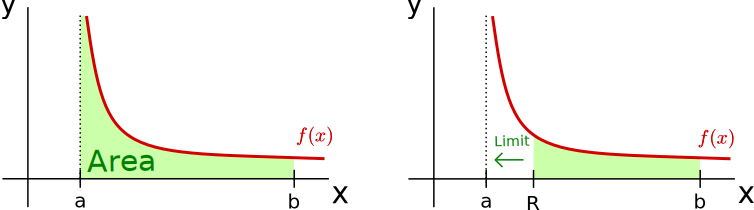
\includegraphics[width=5in]{images2/improper-integral-theory-1}$$ 
% We let $R$ be a fixed number in $(a,b)$. 
% Then by taking the limit as $R$ approaches $a$ from the {\bf right},  we get the improper integral: 
%$$\int_a^b f(x)\,dx:=\lim_{R\to a^+}\int_R^b f(x)\,dx.$$ 
% Now we can apply FTC to the last integral as $f(x)$ is continuous on $[R,b]$.
%
%\begin{example}{A Divergent Integral}{A Divergent Integral}
%Determine if $\ds\int_{-1}^1\frac{1}{x^2}\,dx$ is convergent or divergent.
%\end{example}  
%
%\begin{solution}
% The function $f(x)=1/x^2$ has a discontinuity at $x=0$, which lies in $[-1,1]$.  
% We must compute $\ds\int_{-1}^0 \frac{1}{x^2}\,dx$ and $\ds\int_0^1 \frac{1}{x^2}\,dx$. Let's start with $\ds\int_0^1 \frac{1}{x^2}\,dx$:  
%$$\int_0^1 \frac{1}{x^2}\,dx = \lim_{R\to 0^+} \int_R^1 \frac{1}{x^2} \,dx = \lim_{R\to 0^+} -\frac{1}{x}\bigg|_R^1
%= -1 + \lim_{R\to 0^+} \frac{1}{R}$$
%which diverges to $+\infty$.
% Therefore, $\ds\int_{-1}^1\frac{1}{x^2}\,dx$ is {\bf divergent} since one of $\ds\int_{-1}^0 \frac{1}{x^2}\,dx$ and $\ds\int_0^1 \frac{1}{x^2}\,dx$ is divergent.
%\end{solution}
%
%
%% % % % % % %
%% % The following example 'Integral of the Logarithm' can be replaced with the next example if Integration by Parts is not included in the text adaptation.
%\begin{example}{Integral of the Logarithm}{Integral of the Logarithm}
%Determine if $\ds\int_0^1 \ln x \,dx$ is convergent or divergent. Evaluate it if it is convergent.
%\end{example}  
%
%\begin{solution}
%Note that $f(x)=\ln x$ is discontinuous at the endpoint $x=0$. 
%We first use integration by parts to compute $\ds\int\ln x\,dx$.
%We let $u=\ln x$ and $dv=dx$.
%Then $du=(1/x)dx$, $v=x$, giving:
%\begin{eqnarray*}
%\int \ln x\,dx &=& \ds x\ln x-\int x\cdot\frac{1}{x}\,dx\\
%&=& x\ln x-\int 1\,dx\\
%&=& x\ln x-x+C\\
%\end{eqnarray*}
% Now using the definition of improper integral for $\ds\int_0^1 \ln x \,dx$: 
%$$
%	\int_0^1 \ln x \,dx = \lim_{R\to 0^+} \int_R^1 \ln x\,dx 
%	=  \lim_{R\to 0^+} (x\ln x-x)\bigg|_R^1 
%	%=  \lim_{R\to 0^+} \left(\left[\ln 1-1\right] - \left[R\ln R-R\right]\right)
%	=  -1 - \lim_{R\to 0^+}(R\ln R) + \lim_{R\to 0^+}R 
%$$
%Note that $\ds\lim_{R\to 0^+}R=0$. 
%We next compute $\ds\lim_{R\to 0^+}(R\ln R)$.
%First, we rewrite the expression as follows:
%$$\lim_{x\to0^+}(R\ln R)=\lim_{R\to0^+}\frac{\ln R}{1/R}.$$
%Now the limit is of the indeterminate type $(-\infty)/(\infty)$ and l'H\^opital's Rule can be applied.  
%$$\lim_{R\to0^+}(R\ln R) =\lim_{R\to0^+}\frac{\ln R}{1/R}
%=\lim_{R\to0^+}\frac{1/R}{-1/R^2}
%=\lim_{R\to0^+}-\frac{R^2}{R}
%=\lim_{R\to0^+}(-R)
%=0$$
%Thus, $\ds\lim_{R\to 0^+}(R\ln R)=0$.
%Thus
%$$\int_0^1 \ln x \,dx = -1,$$ 
%and the integral is convergent to $-1$. 
%
%Graphically, one might interpret this to mean that the net area under $\ln x$ on $[0,1]$ is $-1$ (the area in this case lies below the $x$-axis). 
%$$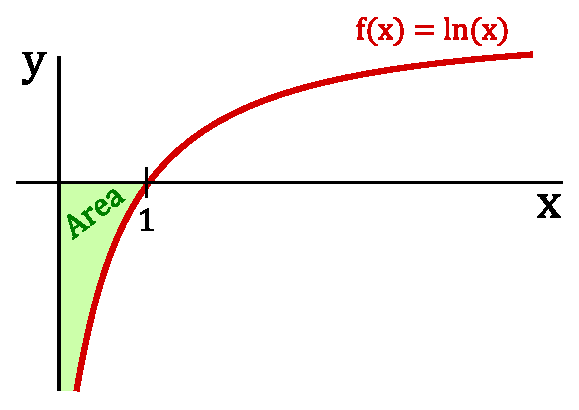
\includegraphics[width=2.5in]{images2/improper-integral-example-2}$$
%\end{solution}
%
%\begin{example}{Integral of a Square Root}{IntSquareRoot}
%Determine if $\ds\int_0^4\frac{dx}{\sqrt{4-x}}$ is convergent or divergent. Evaluate it if it is convergent.
%\end{example}
%\begin{solution}
%Note that $\frac{1}{\sqrt{4-x}}$ is discontinuous at the endpoint $x=4$. We use a $u$-substitution to compute $\int \frac{dx}{\sqrt{4-x}}$. We let $u=4-x$, then $du=-dx$, giving:
%\begin{align*}
%\ds\int\frac{dx}{\sqrt{4-x}}&=\int-\frac{du}{u^{1/2}}	\\
%&=\int -u^{-1/2}\,du	\\
%&=-2(u)^{1/2}+C	\\
%&=-2\sqrt{4-x}+C
%\end{align*}
%Now using the definition of improper integrals for $\ds\int_0^4\frac{dx}{\sqrt{4-x}}$:
%\[\ds\int_0^4\frac{dx}{\sqrt{4-x}}=\lim_{R\to4^{-}}(-2\sqrt{4-x})\bigg|_0^R=\lim_{R\to4^{-}}-2\sqrt{4-R}+2\sqrt{4}=4\]
%\end{solution}
%
%\begin{example}{Improper Integral}{ImpIntExample}
%Determine if $\ds\int_{1}^{2}\dfrac{dx}{\left( x-1\right) ^{1/3}}$ is
%convergent or divergent. Evaluate it if it is convergent.
%\end{example}
%\begin{solution}
%Note that $f\left( x\right) =\dfrac{1}{\left( x-1\right) ^{1/3}}$
%is discontinuous at the endpoint $x=1.$ We first use substitution to find
%$\ds\int \dfrac{dx}{\left( x-1\right) ^{1/3}}.$ We let $u=x-1.$ Then $du=dx,$
%giving%
%\begin{equation*}
%\int \dfrac{dx}{\left( x-1\right) ^{1/3}}=\int \frac{du}{u^{1/3}}=\int
%u^{-1/3}du=\frac{3}{2}u^{2/3}+C=\frac{3}{2}\left( x-1\right) ^{2/3}+C.
%\end{equation*}%
%Now using the definition of improper integral for $\ds\int_{1}^{2}\dfrac{dx}{%
%	\left( x-1\right) ^{1/3}}:$%
%\begin{equation*}
%\int_{1}^{2}\dfrac{dx}{\left( x-1\right) ^{1/3}}=\lim_{R\rightarrow
%	1^{+}}\int_{R}^{2}\dfrac{dx}{\left( x-1\right) ^{1/3}}=\left.
%\lim_{R\rightarrow 1^{+}}\frac{3}{2}\left( x-1\right) ^{2/3}\right\vert
%_{R}^{2}=\frac{3}{2}-\lim_{R\rightarrow 1^{+}}\frac{3}{2}\left( R-1\right)
%^{2/3}=\frac{3}{2},
%\end{equation*}%
%and the integral is convergent to $\frac{3}{2}.$ Graphically, one might
%interpret this to mean that the net area under $\dfrac{1}{\left( x-1\right)
%	^{1/3}}$ on $\left[ 1,2\right] $ is $\frac{3}{2}$.
%
%$$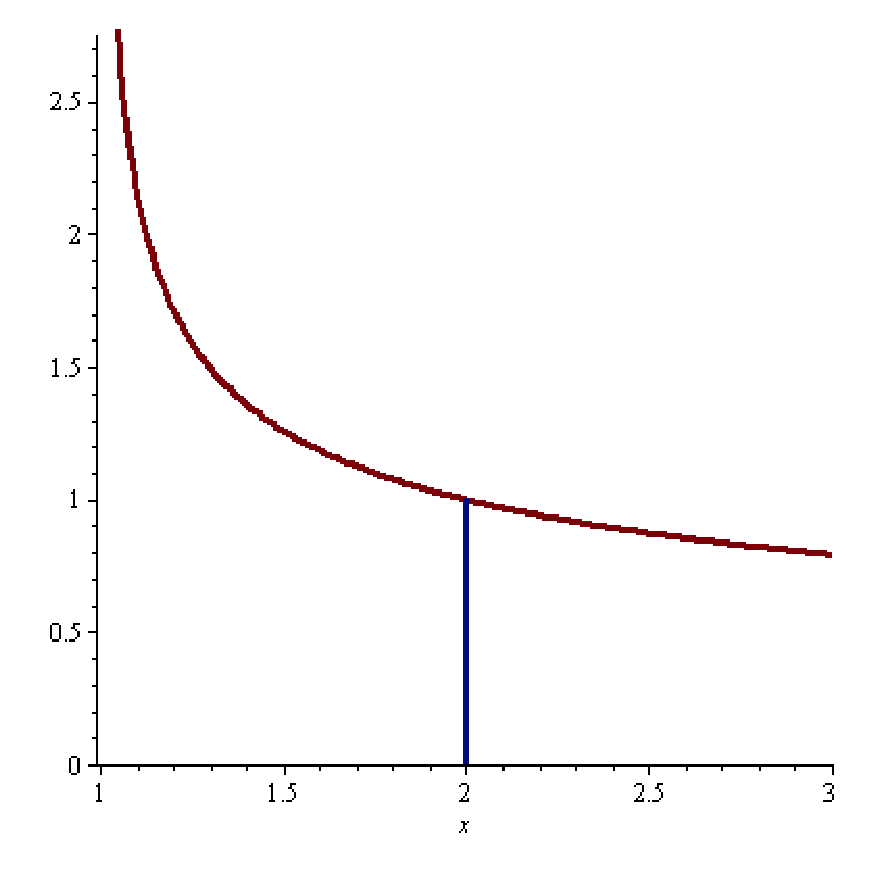
\includegraphics[width=8cm]{images/improper-int-example}$$
%\end{solution}
%
%The following test allows us to determine convergence/divergence information about improper integrals that are hard to compute by comparing them to easier ones. 
%We state the test for $[a,\infty)$, but similar versions hold for the other improper integrals.
%
%\begin{formulabox}[The Comparison Test]
%Assume that $f(x)\geq g(x)\geq 0$ for $x\geq a$.
%\begin{enumerate}[(i)]
%\item	If $\ds\int_a^\infty f(x)\,dx$ {\bf converges}, then $\ds\int_a^\infty g(x)\,dx$ also {\bf converges}.
%\item	If $\ds\int_a^\infty g(x)\,dx$ {\bf diverges}, then $\ds\int_a^\infty f(x)\,dx$ also {\bf diverges}. 
%\end{enumerate}
%\end{formulabox}
%
%Informally, (i) says that if $f(x)$ is larger than $g(x)$, and the area under $f(x)$ is finite (converges), then the area under $g(x)$ must also be finite (converges). 
%Informally, (ii) says that if $f(x)$ is larger than $g(x)$, and the area under $g(x)$ is infinite (diverges), then the area under $f(x)$ must also be infinite (diverges). 
%
%$$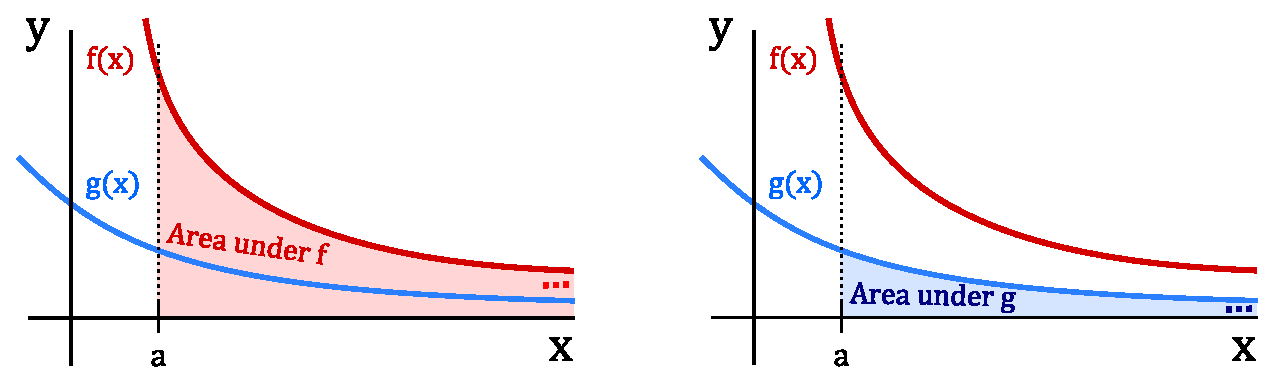
\includegraphics[width=6in]{images2/improper-integral-theory-3}$$
%
%\begin{example}{Comparison Test}{Comparison Test}
%Show that $\ds\int_2^\infty \frac{\cos^2x}{x^2} \,dx$ converges.
%\end{example} 
%
%\begin{solution}
%We use the comparison test to show that it converges. 
%Note that $0\leq \cos^2x\leq 1$ and hence 
%$$0 \leq\frac{\cos^2x}{x^2}\leq\frac{1}{x^2}.$$
%Thus, taking $f(x)=1/x^2$ and $g(x)=\cos^2x / x^2$ we have $f(x)\geq g(x)\geq 0$. 
%One can easily see that $\ds\int_2^\infty \frac{1}{x^2}\,dx$ converges. 
%Therefore, $\ds\int_2^\infty \frac{\cos^2x}{x^2} \,dx$ also converges.
%\end{solution}



We begin this section by considering the following definite integrals:
\begin{itemize}
\item	$\ds \int_0^{100}\frac1{1+x^2}\ dx \approx 1.5608,$
\item	$\ds \int_0^{1000}\frac1{1+x^2}\ dx \approx 1.5698,$
\item	$\ds \int_0^{10,000}\frac1{1+x^2}\ dx \approx 1.5707.$
\end{itemize}

Notice how the integrand is $1/(1+x^2)$ in each integral (which is sketched in Figure \ref{fig:improper1}). As the upper bound gets larger, one would expect the ``area under the curve'' would also grow. While the definite integrals do increase in value as the upper bound grows, they are not  increasing by much. In fact, consider:
$$\int_0^b \frac{1}{1+x^2}\ dx = \tan^{-1}x\Big|_0^b = \tan^{-1}b-\tan^{-1}0 = \tan^{-1}b.$$
As $b\rightarrow \infty$, $\tan^{-1}b \rightarrow \pi/2.$ Therefore it seems that as the upper bound $b$ grows, the value of the definite integral $\ds \int_0^b\frac{1}{1+x^2}\ dx$ approaches $\pi/2\approx 1.5708$. This should strike the reader as being a bit amazing: even though the curve extends ``to infinity,'' it has a finite amount of area underneath it.

\mfigure{.75}{Graphing $\ds f(x)=\frac{1}{1+x^2}$.}{fig:improper1}{
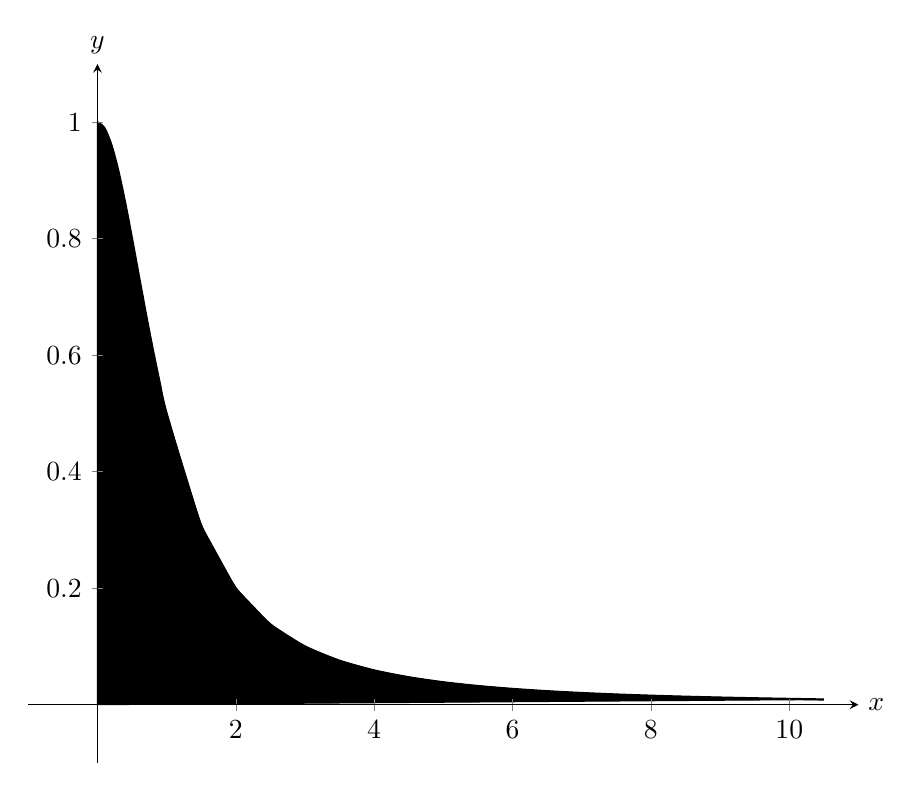
\begin{tikzpicture}
\begin{axis}[width=\textwidth,%
axis y line=middle,axis x line=middle,name=myplot,axis on top,%
			%x=.37\marginparwidth,
			%y=.37\marginparwidth,
%			xtick={-1,1},% 
%			extra x ticks={.5,3},
%			extra x tick labels={$a$,$b$},
%			ytick={-1,1},
			%minor y tick num=1,%extra y ticks={-5,-3,...,7},%
%			minor x tick num=4,
			ymin=-.1,ymax=1.1,%
			xmin=-1,xmax=11%
]

\addplot [{\coloronefill},fill={\coloronefill}] coordinates {(0,1.)(0.1,0.9901)(0.2,0.9615)(0.3,0.9174)(0.4,0.8621)(0.5,0.8)(0.6,0.7353)(0.7,0.6711)(0.8,0.6098)(0.9,0.5525)(1.,0.5)(1.5,0.3077)(2.,0.2)(2.5,0.1379)(3.,0.1)(3.5,0.07547)(4.,0.05882)(4.5,0.04706)(5.,0.03846)(5.5,0.032)(6.,0.02703)(6.5,0.02312)(7.,0.02)(7.5,0.01747)(8.,0.01538)(8.5,0.01365)(9.,0.0122)(9.5,0.01096)(10.,0.009901)(10.5,0.0089)} -- (axis cs:0,0)--cycle;

\addplot [{\colorone},thick,smooth] coordinates {(0,1.)(0.1,0.9901)(0.2,0.9615)(0.3,0.9174)(0.4,0.8621)(0.5,0.8)(0.6,0.7353)(0.7,0.6711)(0.8,0.6098)(0.9,0.5525)(1.,0.5)(1.5,0.3077)(2.,0.2)(2.5,0.1379)(3.,0.1)(3.5,0.07547)(4.,0.05882)(4.5,0.04706)(5.,0.03846)(5.5,0.032)(6.,0.02703)(6.5,0.02312)(7.,0.02)(7.5,0.01747)(8.,0.01538)(8.5,0.01365)(9.,0.0122)(9.5,0.01096)(10.,0.009901)(10.5,0.0089)};

%\filldraw (axis cs:.707,.707) circle (1pt) node [shift={(6pt,11pt)}] {\scriptsize ($\cos \theta$,$\sin \theta$)};
%
%\draw (axis cs:.6,.25) node {\scriptsize $\ds\frac{\theta}{2}$};
%\draw (axis cs:-.75,1) node {\scriptsize $x^2+y^2=1$};

\end{axis}

\node [right] at (myplot.right of origin) { $x$};
\node [above] at (myplot.above origin) { $y$};
\end{tikzpicture}
}

When we defined the definite integral $\ds\int_a^b f(x)\ dx$, we made two stipulations:
	\begin{enumerate}
	\item		The interval over which we integrated, $[a,b]$, was a finite interval, and
	\item		The function $f(x)$ was continuous on $[a,b]$ (ensuring that the range of $f$ was finite).
	\end{enumerate}
	
In this section we consider integrals where one or both of the above conditions do not hold. Such integrals are called \textbf{improper integrals.}

\subsection*{Improper Integrals with Infinite Bounds}

\begin{definition}{Improper Integrals with Infinite Bounds; Converge, Diverge}{def:imp_int1}
{
\begin{enumerate}
\item		Let $f$ be a continuous function on $[a,\infty)$. Define \index{integration!improper}\index{improper integration}\index{convergence!of improper int.}\index{divergence!of improper int.}
$$\small\int_a^\infty f(x)\ dx \quad \text{to be}\quad \lim_{b\to\infty}\int_a^b f(x)\ dx.$$

\item		Let $f$ be a continuous function on $(-\infty,b]$. Define
$$\small\int_{-\infty}^b f(x)\ dx \quad \text{to be}\quad \lim_{a\to-\infty}\int_a^b f(x)\ dx.$$

\item		Let $f$ be a continuous function on $(-\infty,\infty)$. Let $c$ be any real number; define
$$\small\int_{-\infty}^\infty f(x)\ dx \quad \text{to be}\quad \lim_{a\to-\infty}\int_a^c f(x)\ dx\ +\ \lim_{b\to\infty}\int_c^b f(x)\ dx.$$
\end{enumerate}
An improper integral is said to \textbf{converge} if its corresponding limit exists; otherwise, it \textbf{diverges}. The improper integral in part 3 converges if and only if both of its limits exist.
}
\end{definition}


\begin{example}{Evaluating improper integrals}{ex_impint1}
{
Evaluate the following improper integrals.\\
\noindent%
\begin{minipage}[t]{.5\textwidth}
\begin{enumerate}
\item		$\ds\int_1^\infty \frac1{x^2}\ dx$
\item		$\ds\int_1^\infty \frac1x\ dx$
\end{enumerate}
\end{minipage}
\begin{minipage}[t]{.5\textwidth}
\begin{enumerate}\addtocounter{enumi}{2}
\item		$\ds\int_{-\infty}^0 e^x\ dx$
\item		$\ds\int_{-\infty}^\infty \frac1{1+x^2}\ dx$
\end{enumerate}
\end{minipage}
}
\end{example}

\begin{solution}
{\begin{enumerate}
\item		\hfill$\begin{aligned}[t] \int_1^\infty \frac{1}{x^2}\ dx\  =\ \lim_{b\to\infty} \int_1^b\frac1{x^2}\ dx\  &=\ \lim_{b\to\infty} \frac{-1}{x}\Big|_1^b \\ 
 %&= \lim_{b\to\infty} \frac{-1}{x}\Big|_1^b \\
 &= \lim_{b\to\infty} \frac{-1}{b} + 1\\
 &= 1.\end{aligned}$\hfill\null

A graph of the area defined by this integral is given in Figure \ref{fig:impint1a}.
 
\mfigure{.7}{A graph of $f(x) = \frac{1}{x^2}$ in Example \ref{exa:ex_impint1}.}{fig:impint1a}{
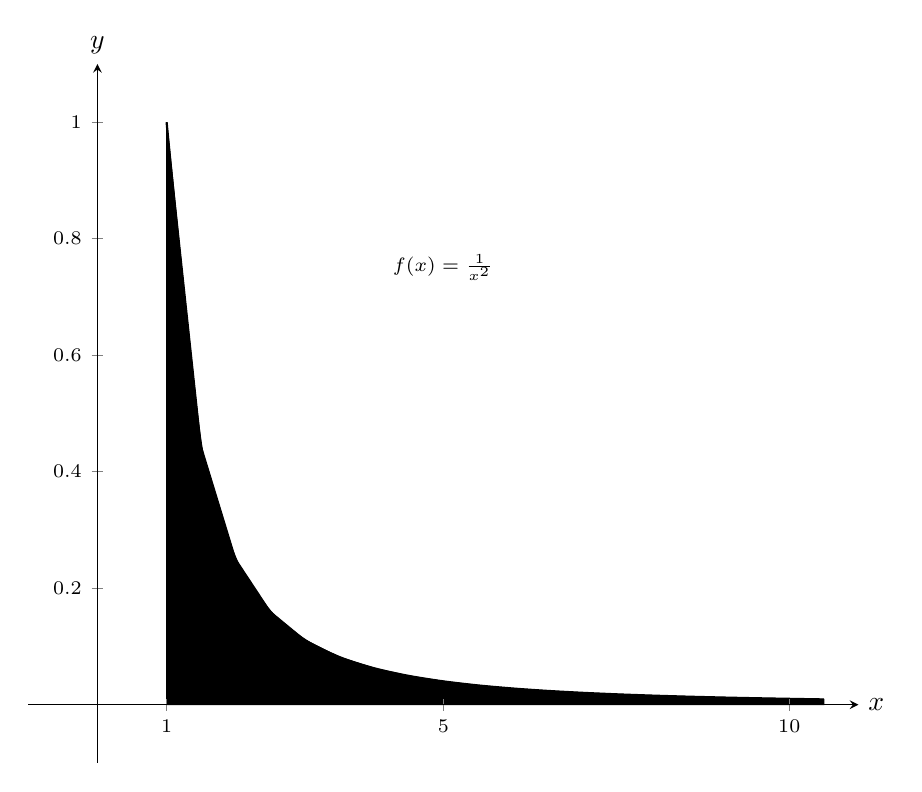
\begin{tikzpicture}
\begin{axis}[width=\textwidth,%
tick label style={font=\scriptsize},axis y line=middle,axis x line=middle,name=myplot,axis on top,%
			%x=.37\marginparwidth,
			%y=.37\marginparwidth,
			xtick={1,5,10},% 
%			extra x ticks={.5,3},
%			extra x tick labels={$a$,$b$},
%			ytick={-1,1},
			%minor y tick num=1,%extra y ticks={-5,-3,...,7},%
%			minor x tick num=4,
			ymin=-.1,ymax=1.1,%
			xmin=-1,xmax=11%
]

\addplot [{\coloronefill},fill={\coloronefill}] coordinates {(1.,1.)(1.5,0.4444)(2.,0.25)(2.5,0.16)(3.,0.1111)(3.5,0.08163)(4.,0.0625)(4.5,0.04938)(5.,0.04)(5.5,0.03306)(6.,0.02778)(6.5,0.02367)(7.,0.02041)(7.5,0.01778)(8.,0.01563)(8.5,0.01384)(9.,0.01235)(9.5,0.01108)(10.,0.01)(10.5,0.009)} -- (axis cs:10.5,0)--(axis cs:1,0)--cycle;

\addplot [{\colorone},thick,smooth] coordinates {(1.,1.)(1.5,0.4444)(2.,0.25)(2.5,0.16)(3.,0.1111)(3.5,0.08163)(4.,0.0625)(4.5,0.04938)(5.,0.04)(5.5,0.03306)(6.,0.02778)(6.5,0.02367)(7.,0.02041)(7.5,0.01778)(8.,0.01563)(8.5,0.01384)(9.,0.01235)(9.5,0.01108)(10.,0.01)(10.5,0.009)};

\draw (axis cs:5,.75) node {\scriptsize $\ds f(x)=\frac{1}{x^2}$};

\end{axis}

\node [right] at (myplot.right of origin) { $x$};
\node [above] at (myplot.above origin) { $y$};
\end{tikzpicture}
}
 
\item		\hfill$\begin{aligned}[t]%
			\int_1^\infty \frac1x\ dx & = \lim_{b\to\infty}\int_1^b\frac1x\ dx \\
						&= \lim_{b\to\infty} \ln |x|\Big|_1^b \\
						&= \lim_{b\to\infty} \ln (b)\\
						&= \infty.
	\end{aligned}$\hfill\null
	
The limit does not exist, hence the improper integral $\ds\int_1^\infty\frac1x\ dx$ diverges. Compare the graphs in Figures \ref{fig:impint1a} and \ref{fig:impint1b}; notice how the graph of $f(x) = 1/x$ is noticeably larger. This difference is enough to cause the improper integral to diverge.

\mfigure{.8}{A graph of $f(x) = \frac{1}{x}$ in Example \ref{exa:ex_impint1}.}{fig:impint1b}{
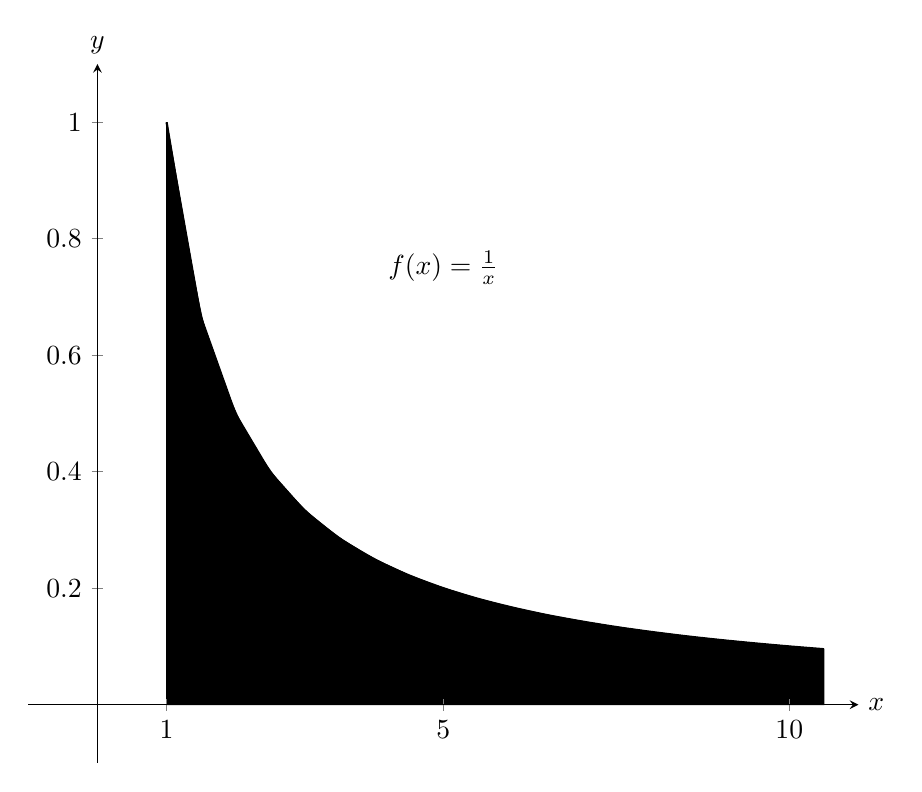
\begin{tikzpicture}
\begin{axis}[width=\textwidth,%
axis y line=middle,axis x line=middle,name=myplot,axis on top,%
			%x=.37\marginparwidth,
			%y=.37\marginparwidth,
			xtick={1,5,10},% 
%			extra x ticks={.5,3},
%			extra x tick labels={$a$,$b$},
%			ytick={-1,1},
			%minor y tick num=1,%extra y ticks={-5,-3,...,7},%
%			minor x tick num=4,
			ymin=-.1,ymax=1.1,%
			xmin=-1,xmax=11%
]

\addplot [{\coloronefill},fill={\coloronefill}] coordinates {(1.,1.)(1.5,0.6667)(2.,0.5)(2.5,0.4)(3.,0.3333)(3.5,0.2857)(4.,0.25)(4.5,0.2222)(5.,0.2)(5.5,0.1818)(6.,0.1667)(6.5,0.1538)(7.,0.1429)(7.5,0.1333)(8.,0.125)(8.5,0.1176)(9.,0.1111)(9.5,0.1053)(10.,0.1)(10.5,0.09524)} -- (axis cs:10.5,0)-- (axis cs:1,0)--cycle;

\addplot [{\colorone},thick,smooth] coordinates {(1.,1.)(1.5,0.6667)(2.,0.5)(2.5,0.4)(3.,0.3333)(3.5,0.2857)(4.,0.25)(4.5,0.2222)(5.,0.2)(5.5,0.1818)(6.,0.1667)(6.5,0.1538)(7.,0.1429)(7.5,0.1333)(8.,0.125)(8.5,0.1176)(9.,0.1111)(9.5,0.1053)(10.,0.1)(10.5,0.09524)};

\draw (axis cs:5,.75) node { $\ds f(x)=\frac{1}{x}$};
\end{axis}

\node [right] at (myplot.right of origin) { $x$};
\node [above] at (myplot.above origin) { $y$};
\end{tikzpicture}
}

\item		\hfill$\begin{aligned}[t]%
			\int_{-\infty}^0 e^x \ dx &= \lim_{a\to-\infty} \int_a^0e^x\ dx \\
					&=  \lim_{a\to-\infty} e^x\Big|_a^0 \\
					&= \lim_{a\to-\infty} e^0-e^a \\
					&= 1.
		\end{aligned}$\hfill\null
		
		A graph of the area defined by this integral is given in Figure \ref{fig:impint1c}.
		
\mfigure{.55}{A graph of $f(x) = e^x$ in Example \ref{exa:ex_impint1}.}{fig:impint1c}{
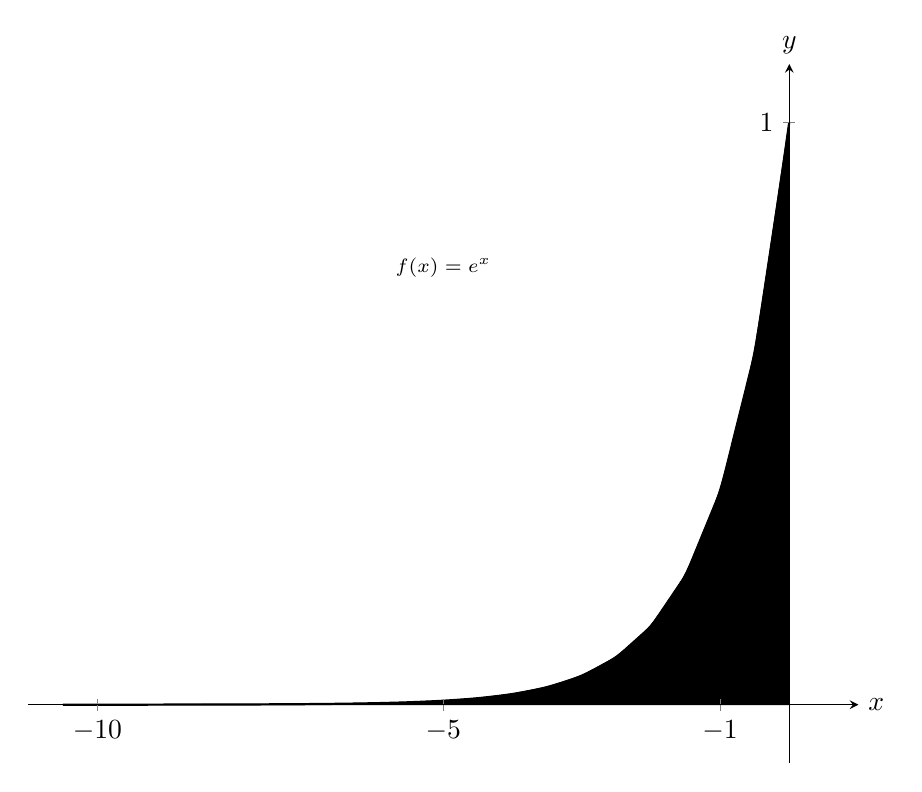
\begin{tikzpicture}
\begin{axis}[width=\textwidth,%
axis y line=middle,axis x line=middle,name=myplot,axis on top,%
			%x=.37\marginparwidth,
			%y=.37\marginparwidth,
			xtick={-1,-5,-10},%
%			extra x ticks={.5,3},
%			extra x tick labels={$a$,$b$},
			ytick={1},
			%minor y tick num=1,%extra y ticks={-5,-3,...,7},%
%			minor x tick num=4,
			ymin=-.1,ymax=1.1,%
			xmin=-11,xmax=1%
]

\addplot [{\coloronefill},fill={\coloronefill}] coordinates {(-10.5,0)(-10.,0)(-9.5,0)(-9.,0.0001234)(-8.5,0.0002035)(-8.,0.0003355)(-7.5,0.0005531)(-7.,0.0009119)(-6.5,0.001503)(-6.,0.002479)(-5.5,0.004087)(-5.,0.006738)(-4.5,0.01111)(-4.,0.01832)(-3.5,0.0302)(-3.,0.04979)(-2.5,0.08208)(-2.,0.1353)(-1.5,0.2231)(-1.,0.3679)(-0.5,0.6065)(0,1.)} -- (axis cs:0,0)--cycle;

\addplot [{\colorone},thick,smooth] coordinates {(-10.5,0)(-10.,0)(-9.5,0)(-9.,0.0001234)(-8.5,0.0002035)(-8.,0.0003355)(-7.5,0.0005531)(-7.,0.0009119)(-6.5,0.001503)(-6.,0.002479)(-5.5,0.004087)(-5.,0.006738)(-4.5,0.01111)(-4.,0.01832)(-3.5,0.0302)(-3.,0.04979)(-2.5,0.08208)(-2.,0.1353)(-1.5,0.2231)(-1.,0.3679)(-0.5,0.6065)(0,1.)};

\draw (axis cs:-5,.75) node {\scriptsize $\ds f(x)=e^x$};
\end{axis}

\node [right] at (myplot.right of origin) { $x$};
\node [above] at (myplot.above origin) { $y$};
\end{tikzpicture}
}

\item		We will need to break this into two improper integrals and choose a value of $c$ as in part 3 of Definition \ref{def:imp_int1}. Any value of $c$ is fine; we choose $c=0$.

\begin{align*}%
		\int_{-\infty}^\infty \frac1{1+x^2}\ dx &= \lim_{a\to-\infty} \int_a^0\frac{1}{1+x^2}\ dx + \lim_{b\to\infty} \int_0^b\frac{1}{1+x^2}\ dx \\
						&= \lim_{a\to-\infty} \tan^{-1}x\Big|_a^0 + \lim_{b\to\infty} \tan^{-1}x\Big|_0^b\\
						&= \lim_{a\to-\infty} \left(\tan^{-1}0-\tan^{-1}a\right) + \lim_{b\to\infty} \left(\tan^{-1}b-\tan^{-1}0\right)\\		
						&= \left(0-\frac{-\pi}2\right) + \left(\frac{\pi}2-0\right).\\
						\intertext{Each	limit exists, hence the original integral converges and has value:}
						&= \pi.
\end{align*}
%\enlargethispage{2\baselineskip}
A graph of the area defined by this integral is given in Figure \ref{fig:impint1d}.

\mfigure{.8}{A graph of $f(x) = \frac{1}{1+x^2}$ in Example \ref{exa:ex_impint1}.}{fig:impint1d}{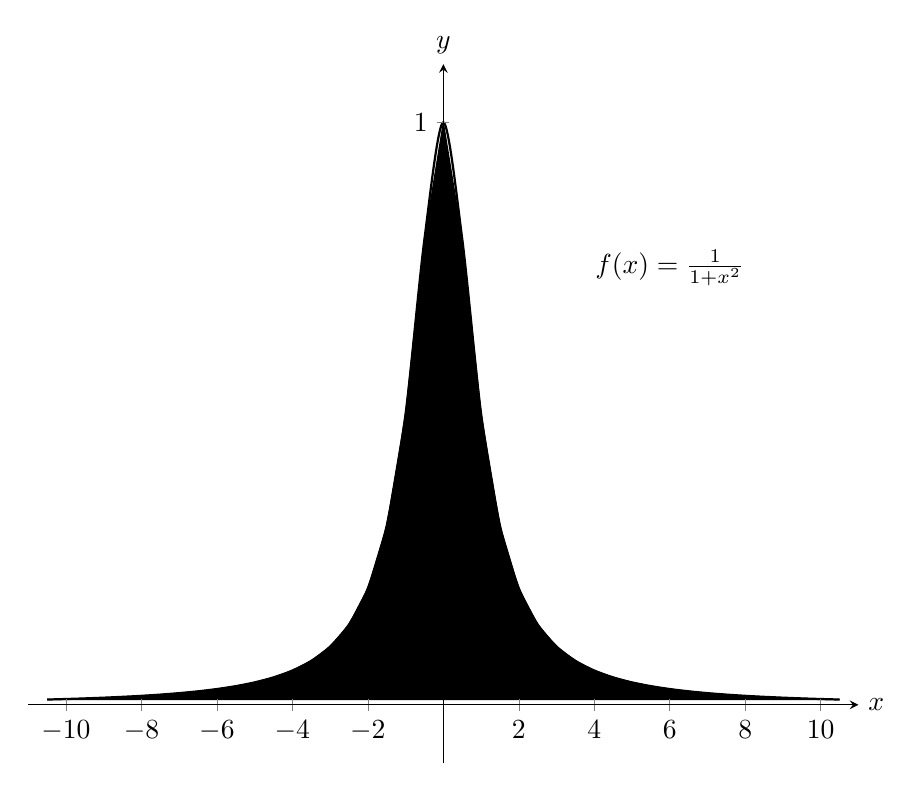
\begin{tikzpicture}
\begin{axis}[width=\textwidth,%
axis y line=middle,axis x line=middle,name=myplot,axis on top,%
			%x=.37\marginparwidth,
			%y=.37\marginparwidth,
%			xtick={-1,-5,-10},%
%			extra x ticks={.5,3},
%			extra x tick labels={$a$,$b$},
			ytick={1},
			%minor y tick num=1,%extra y ticks={-5,-3,...,7},%
%			minor x tick num=4,
			ymin=-.1,ymax=1.1,%
			xmin=-11,xmax=11%
]

\addplot [{\coloronefill},fill={\coloronefill}] coordinates {(-10.5,0.008989)(-10.,0.009901)(-9.5,0.01096)(-9.,0.0122)(-8.5,0.01365)(-8.,0.01538)(-7.5,0.01747)(-7.,0.02)(-6.5,0.02312)(-6.,0.02703)(-5.5,0.032)(-5.,0.03846)(-4.5,0.04706)(-4.,0.05882)(-3.5,0.07547)(-3.,0.1)(-2.5,0.1379)(-2.,0.2)(-1.5,0.3077)(-1.,0.5)(-0.5,0.8)(0,1.)(0.5,0.8)(1.,0.5)(1.5,0.3077)(2.,0.2)(2.5,0.1379)(3.,0.1)(3.5,0.07547)(4.,0.05882)(4.5,0.04706)(5.,0.03846)(5.5,0.032)(6.,0.02703)(6.5,0.02312)(7.,0.02)(7.5,0.01747)(8.,0.01538)(8.5,0.01365)(9.,0.0122)(9.5,0.01096)(10.,0.009901)(10.5,0.008989)} --cycle;

\addplot [{\colorone},thick,smooth] coordinates {(-10.5,0.008989)(-10.,0.009901)(-9.5,0.01096)(-9.,0.0122)(-8.5,0.01365)(-8.,0.01538)(-7.5,0.01747)(-7.,0.02)(-6.5,0.02312)(-6.,0.02703)(-5.5,0.032)(-5.,0.03846)(-4.5,0.04706)(-4.,0.05882)(-3.5,0.07547)(-3.,0.1)(-2.5,0.1379)(-2.,0.2)(-1.5,0.3077)(-1.,0.5)(-0.5,0.8)(0,1.)(0.5,0.8)(1.,0.5)(1.5,0.3077)(2.,0.2)(2.5,0.1379)(3.,0.1)(3.5,0.07547)(4.,0.05882)(4.5,0.04706)(5.,0.03846)(5.5,0.032)(6.,0.02703)(6.5,0.02312)(7.,0.02)(7.5,0.01747)(8.,0.01538)(8.5,0.01365)(9.,0.0122)(9.5,0.01096)(10.,0.009901)(10.5,0.008989)};

\draw (axis cs:6,.75) node { $\ds f(x)=\frac{1}{1+x^2}$};
\end{axis}

\node [right] at (myplot.right of origin) { $x$};
\node [above] at (myplot.above origin) { $y$};
\end{tikzpicture}
}
\end{enumerate}
\vskip-\baselineskip
}
\end{solution}







The previous section introduced l'H\^opital's Rule, a method of evaluating limits that return indeterminate forms. It is not uncommon for the limits resulting from improper integrals to need this rule as demonstrated next.\\


\begin{example}{Improper integration and l'H\^opital's Rule}{ex_impint2}
{
Evaluate the improper integral $\ds \int_1^\infty \frac{\ln x}{x^2}\ dx.$}
\end{example}


\begin{solution}
{This integral will require the use of Integration by Parts. Let $u = \ln x$ and $dv = 1/x^2\ dx$. Then
\mfigure{.6}{A graph of $f(x) = \frac{\ln x}{x^2}$ in Example \ref{exa:ex_impint2}.}{fig:impint2}{
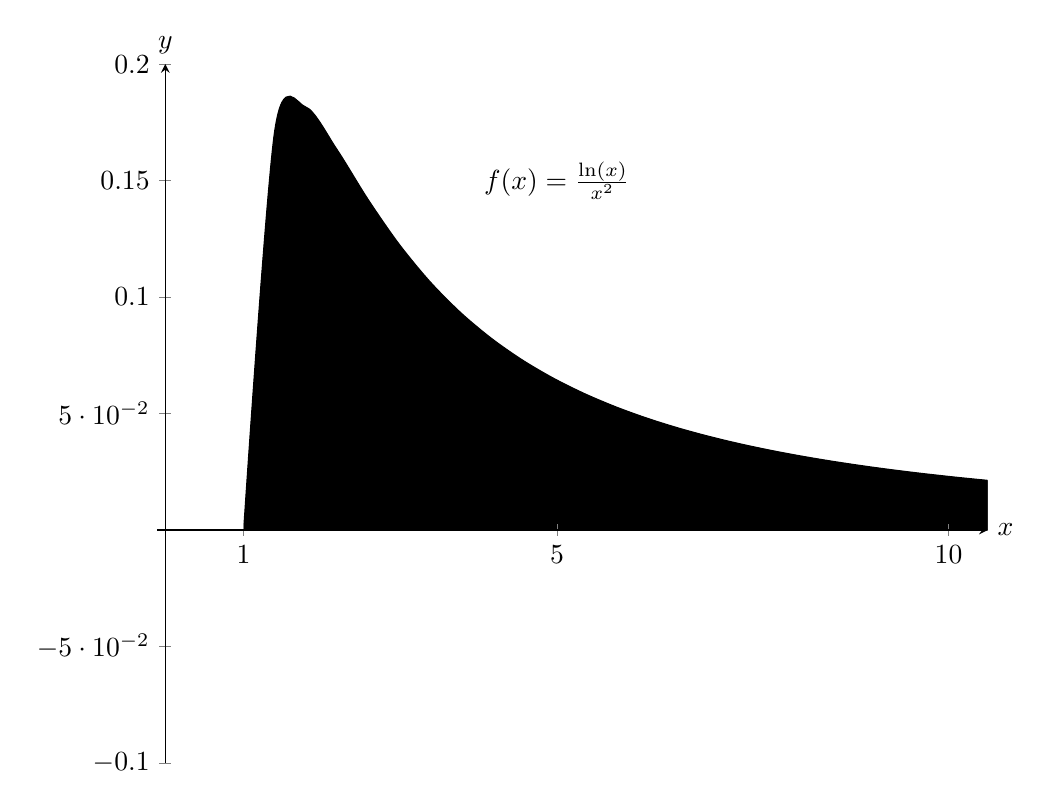
\begin{tikzpicture}
\begin{axis}[width=\textwidth,%
axis y line=middle,axis x line=middle,name=myplot,axis on top,%
			%x=.37\marginparwidth,
			%y=.37\marginparwidth,
			xtick={1,5,10},%
%			extra x ticks={.5,3},
%			extra x tick labels={$a$,$b$},
%			ytick={1},
			%minor y tick num=1,%extra y ticks={-5,-3,...,7},%
%			minor x tick num=4,
			ymin=-.1,ymax=.2,%
			xmin=-.1,xmax=10.5%
]

%\addplot [{\coloronefill},fill={\coloronefill}] coordinates {(0.1,3.162)(0.2,2.236)(0.3,1.826)(0.4,1.581)(0.5,1.414)(0.6,1.291)(0.7,1.195)(0.8,1.118)(0.9,1.054)(1.,1.)} -- (axis cs:1,0)--(axis cs:.1,0)--cycle;

\addplot [smooth,\colorone, fill={\coloronefill},area style,domain=1:10.5] {(ln(x))/(x^2)} \closedcycle;

%\addplot [{\colorone},thick,smooth] coordinates {(0.1,3.162)(0.2,2.236)(0.3,1.826)(0.4,1.581)(0.5,1.414)(0.6,1.291)(0.7,1.195)(0.8,1.118)(0.9,1.054)(1.,1.)};

\draw (axis cs:5,.15) node {$\ds f(x)=\frac{\ln(x)}{x^2}$};
\end{axis}

\node [right] at (myplot.right of origin) { $x$};
\node [above] at (myplot.above origin) {$y$};
\end{tikzpicture}
}
\begin{align*}
\int_1^\infty\frac{\ln x}{x^2}\ dx &= \lim_{b\to\infty}\int_1^b\frac{\ln x}{x^2}\ dx \\
			&=  \lim_{b\to\infty}\left(-\frac{\ln x}{x}\Big|_1^b +\int_1^b \frac{1}{x^2} \ dx \right)\\
			&=  \lim_{b\to\infty} \left.\left(-\frac{\ln x}{x} -\frac1x\right)\right|_1^b\\
			&=	\lim_{b\to\infty} \left(-\frac{\ln b}{b}-\frac1b - \left(-\ln 1-1\right)\right).\\
			\intertext{The $1/b$ and $\ln 1$ terms go to 0, leaving $\ds \lim_{b\to\infty} -\frac{\ln b}b + 1.$ We need to evaluate $\ds \lim_{b\to\infty} \frac{\ln b}{b}$ with l'H\^opital's Rule. We have:}
		\lim_{b\to\infty}\frac{\ln b}b &\stackrel{\ \text{ by LHR \rule[-5pt]{0pt}{3pt}} \ }{=} \lim_{b\to\infty} \frac{1/b}{1} \\
		&= 0.
\intertext{Thus the improper integral evaluates as: }
\int_1^\infty\frac{\ln x}{x^2}\ dx &= 1.
\end{align*}
}
\end{solution}




\subsection*{Improper Integrals with Infinite Range}

We have just considered definite integrals where the interval of integration was infinite. We now consider another type of improper integration, where the range of the integrand is infinite.


\begin{definition}{Improper Integration with Infinite Range}{def:imp_int2}
{Let $f(x)$ be a continuous function on $[a,b]$ except at $c$, $a\leq c\leq b$, where $x=c$ is a vertical asymptote of $f$. Define\index{integration!improper}\index{improper integration}
$$\int_a^b f(x)\ dx = \lim_{t\to c^-}\int_a^t f(x)\ dx + \lim_{t\to c^+}\int_t^b f(x)\ dx.$$
Again, the integral converges if both limits exist and diverges otherwise.
} 
\end{definition}


\begin{example}{Improper integration of functions with infinite range}{ex_impint3}
{
Evaluate the following improper integrals:
\vskip 10pt
$\ds 1.\ \int_0^1\frac1{\sqrt{x}}\ dx \hskip 50pt 2. \ \int_{-1}^1\frac{1}{x^2}\ dx.$
}
\end{example}


\begin{solution}
{\begin{enumerate}
\item		A graph of $f(x) = 1/\sqrt{x}$ is given in Figure \ref{fig:impint3}. Notice that $f$ has a vertical asymptote at $x=0$; in some sense, we are trying to compute the area of a region that has no ``top.'' Could this have a finite value? 
\begin{align*} \int_0^1 \frac{1}{\sqrt{x}}\ dx &= \lim_{a\to0^+}\int_a^1 \frac1{\sqrt{x}}\ dx \\
			&=	\lim_{a\to0^+} 2\sqrt{x}\Big|_a^1 \\
			&= \lim_{a\to0^+} 2\left(\sqrt{1}-\sqrt{a}\right)\\
			&=	2.
\end{align*}
It turns out that the region does have a finite area even though it has no upper bound (strange things can occur in mathematics when considering the infinite).

{\textbf{Note:} In Definition \ref{def:imp_int2}, $c$ can be one of the endpoints ($a$ or $b$). In that case, there is only one limit to consider as part of the definition.}

\mfigure{.65}{A graph of $f(x)=\frac{1}{\sqrt{x}}$ in Example \ref{exa:ex_impint3}.}{fig:impint3}{
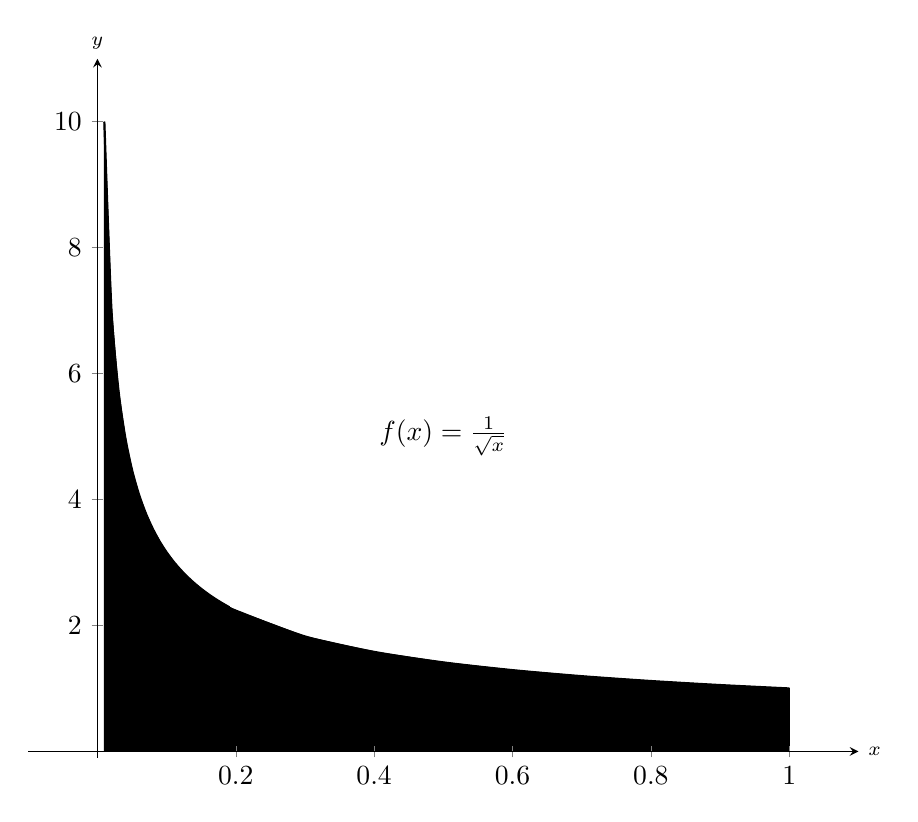
\begin{tikzpicture}
\begin{axis}[width=\textwidth,%
axis y line=middle,axis x line=middle,name=myplot,axis on top,%
			%x=.37\marginparwidth,
			%y=.37\marginparwidth,
%			xtick={1,5,10},%
%			extra x ticks={.5,3},
%			extra x tick labels={$a$,$b$},
%			ytick={1},
			%minor y tick num=1,%extra y ticks={-5,-3,...,7},%
%			minor x tick num=4,
			ymin=-.1,ymax=11,%
			xmin=-.1,xmax=1.1%
]

\addplot [{\coloronefill},fill={\coloronefill}] coordinates {(0.01,10.)(0.02,7.071)(0.03,5.774)(0.04,5.)(0.05,4.472)(0.06,4.082)(0.07,3.78)(0.08,3.536)(0.09,3.333)(0.1,3.162)(0.11,3.015)(0.12,2.887)(0.13,2.774)(0.14,2.673)(0.15,2.582)(0.16,2.5)(0.17,2.425)(0.18,2.357)(0.19,2.294)(0.2,2.236)(0.3,1.826)(0.4,1.581)(0.5,1.414)(0.6,1.291)(0.7,1.195)(0.8,1.118)(0.9,1.054)(1.,1.)} -- (axis cs:1,0)--(axis cs:.01,0)--cycle;

\addplot [{\colorone},thick,smooth] coordinates {(0.01,10.)(0.02,7.071)(0.03,5.774)(0.04,5.)(0.05,4.472)(0.06,4.082)(0.07,3.78)(0.08,3.536)(0.09,3.333)(0.1,3.162)(0.11,3.015)(0.12,2.887)(0.13,2.774)(0.14,2.673)(0.15,2.582)(0.16,2.5)(0.17,2.425)(0.18,2.357)(0.19,2.294)(0.2,2.236)(0.3,1.826)(0.4,1.581)(0.5,1.414)(0.6,1.291)(0.7,1.195)(0.8,1.118)(0.9,1.054)(1.,1.)};

\draw (axis cs:.5,5) node { $\ds f(x)=\frac{1}{\sqrt{x}}$};
\end{axis}

\node [right] at (myplot.right of origin) {\scriptsize $x$};
\node [above] at (myplot.above origin) {\scriptsize $y$};
\end{tikzpicture}
}

\item		The function $f(x) = 1/x^2$ has a vertical asymptote at $x=0$, as shown in Figure \ref{fig:impint3b}, so this integral is an improper integral. Let's eschew using limits for a moment and proceed without recognizing the improper nature of the integral. This leads to:
\begin{align*}
\int_{-1}^1\frac1{x^2}\ dx &= -\frac1x\Big|_{-1}^1\\
			&= -1 - (1)\\
			&=-2 !
\end{align*}
\mfigure{.6}{A graph of $f(x)=\frac{1}{x^2}$ in Example \ref{exa:ex_impint3}.}{fig:impint3b}{
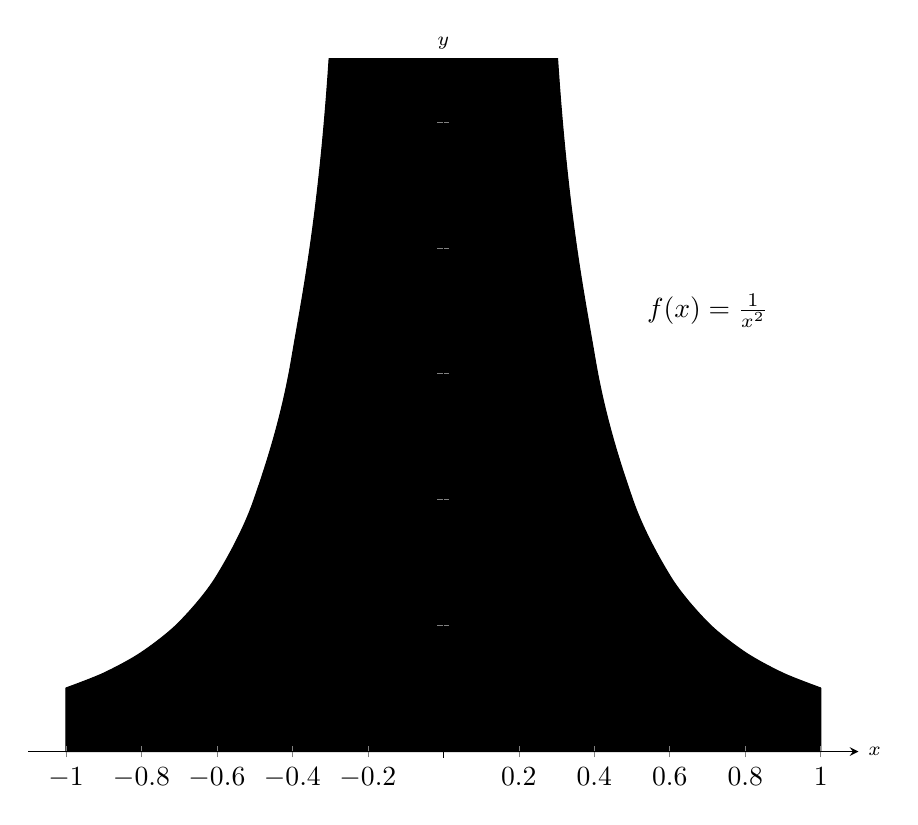
\begin{tikzpicture}
\begin{axis}[width=\textwidth,%
axis y line=middle,axis x line=middle,name=myplot,axis on top,%
			%x=.37\marginparwidth,
			%y=.37\marginparwidth,
%			xtick={.1,.5,1},%
%			extra x ticks={.5,3},
%			extra x tick labels={$a$,$b$},
%			ytick={1},
			%minor y tick num=1,%extra y ticks={-5,-3,...,7},%
%			minor x tick num=4,
			ymin=-.1,ymax=11,%
			xmin=-1.1,xmax=1.1%
]

\addplot [{\coloronefill},fill={\coloronefill},smooth] coordinates {(-1.,1.)(-0.9,1.235)(-0.8,1.563)(-0.7,2.041)(-0.6,2.778)(-0.5,4.)(-0.4,6.25)(-0.3,11.11)(-0.2,25.)} -- (axis cs:0,11)--(axis cs:0,0)--(axis cs:-1,0) --cycle;

\addplot [{\colorone},thick,smooth] coordinates {(-1.,1.)(-0.9,1.235)(-0.8,1.563)(-0.7,2.041)(-0.6,2.778)(-0.5,4.)(-0.4,6.25)(-0.3,11.11)(-0.2,25.)};

\addplot [{\coloronefill},fill={\coloronefill},smooth] coordinates {(0.2,25.)(0.3,11.11)(0.4,6.25)(0.5,4.)(0.6,2.778)(0.7,2.041)(0.8,1.563)(0.9,1.235)(1.,1.)} -- (axis cs:1,0)--(axis cs:0,0)--(axis cs:0,11) --cycle;

\addplot [{\colorone},thick,smooth] coordinates {(0.2,25.)(0.3,11.11)(0.4,6.25)(0.5,4.)(0.6,2.778)(0.7,2.041)(0.8,1.563)(0.9,1.235)(1.,1.)};

\draw (axis cs:.7,7) node { $\ds f(x)=\frac{1}{x^2}$};
\end{axis}

\node [right] at (myplot.right of origin) {\scriptsize $x$};
\node [above] at (myplot.above origin) {\scriptsize $y$};
\end{tikzpicture}
}
Clearly the area in question is above the $x$-axis, yet the area is supposedly negative! Why does our answer not match our intuition? To answer this, evaluate the integral using Definition \ref{def:imp_int2}.
\begin{align*}
\int_{-1}^1\frac1{x^2}\ dx &= \lim_{t\to0^-}\int_{-1}^t \frac1{x^2}\ dx + \lim_{t\to0^+}\int_t^1\frac1{x^2}\ dx \\
			&= \lim_{t\to0^-}-\frac1x\Big|_{-1}^t + \lim_{t\to0^+}-\frac1x\Big|_t^1\\
			&= \lim_{t\to0^-}-\frac1t-1 + \lim_{t\to0^+} -1+\frac1t\\
			&\Rightarrow \Big(\infty-1\Big)\ + \ \Big(- 1+\infty\Big).
\end{align*}
Neither limit converges hence the original improper integral diverges. The nonsensical answer we obtained by ignoring the improper nature of the integral is just that: nonsensical.
%\mnote{.8}{\textbf{Note:} In Example \ref{ex_impint3}, \#2, the final line of calculation states:
%$$\text{``}(\infty-1)+(-\infty-1)\text{.''}$$ 
%Each parenthetical statement stands alone and is the result of an individual limit. We are \textit{not} dealing with the indeterminate form ``$\infty-\infty$'' as the ``infinities'' do not originate from one limit.}
\end{enumerate}
}
\end{solution}




\subsection*{ Understanding Convergence and Divergence}

Oftentimes we are interested in knowing simply whether or not an improper integral converges, and not necessarily the value of a convergent integral. We provide here several tools that help determine the convergence or divergence of improper integrals without integrating.

Our first tool is to understand the behavior of functions of the form $\ds \frac1{x\hskip1pt ^p}$.\\

\begin{example}{Improper integration of $1/x^p$}{ex_impint4}
{
Determine the values of $p$ for which $\ds \int_1^\infty \frac1{x\hskip1pt ^p}\ dx$ converges.
}
\end{example}


\begin{solution}
{We begin by integrating and then evaluating the limit.
\begin{align*}
\int_1^\infty \frac1{x\hskip1pt ^p}\ dx &=	\lim_{b\to\infty}\int_1^b\frac1{x\hskip1pt ^p}\ dx\\
		&=	\lim_{b\to\infty}\int_1^b x^{-p}\ dx \qquad \text{\small (assume $p\neq 1$)}\\
		&= \lim_{b\to\infty} \frac{1}{-p+1}x^{-p+1}\Big|_1^b\\
		&= \lim_{b\to\infty} \frac{1}{1-p}\big(b\hskip1pt^{1-p}-1^{1-p}\big).\\
\end{align*}
When does this limit converge -- i.e., when is this limit \textit{not} $\infty$? This limit converges precisely when the power of $b$ is less than 0: when $1-p<0 \Rightarrow 1<p$. 

\mfigure{.75}{Plotting functions of the form $1/x\,^p$ in Example \ref{exa:ex_impint4}.}{fig:impint4}{
\begin{tikzpicture}
\begin{axis}[width=\textwidth,%
axis y line=middle,axis x line=middle,name=myplot,axis on top,%
			%x=.37\marginparwidth,
			%y=.37\marginparwidth,
			xtick={1},%
%			extra x ticks={.5,3},
%			extra x tick labels={$a$,$b$},
			ytick=\empty,
			%minor y tick num=1,%extra y ticks={-5,-3,...,7},%
%			minor x tick num=4,
			ymin=-.1,ymax=6,%
			xmin=-.1,xmax=2.1%
]

\addplot [dashed,thick,smooth] coordinates {(0.1,10.)(0.15,6.667)(0.2,5.)(0.25,4.)(0.3,3.333)(0.35,2.857)(0.4,2.5)(0.45,2.222)(0.5,2.)(0.55,1.818)(0.6,1.667)(0.65,1.538)(0.7,1.429)(0.75,1.333)(0.8,1.25)(0.85,1.176)(0.9,1.111)(0.95,1.053)(1.,1.)(1.05,0.9524)(1.1,0.9091)(1.15,0.8696)(1.2,0.8333)(1.25,0.8)(1.3,0.7692)(1.35,0.7407)(1.4,0.7143)(1.45,0.6897)(1.5,0.6667)(1.55,0.6452)(1.6,0.625)(1.65,0.6061)(1.7,0.5882)(1.75,0.5714)(1.8,0.5556)(1.85,0.5405)(1.9,0.5263)(1.95,0.5128)(2.,0.5)};

\addplot [{\colorone},thick,smooth] coordinates {(0.1,31.62)(0.15,17.21)(0.2,11.18)(0.25,8.)(0.3,6.086)(0.35,4.829)(0.4,3.953)(0.45,3.313)(0.5,2.828)(0.55,2.452)(0.6,2.152)(0.65,1.908)(0.7,1.707)(0.75,1.54)(0.8,1.398)(0.85,1.276)(0.9,1.171)(0.95,1.08)(1.,1.)(1.05,0.9294)(1.1,0.8668)(1.15,0.8109)(1.2,0.7607)(1.25,0.7155)(1.3,0.6747)(1.35,0.6375)(1.4,0.6037)(1.45,0.5727)(1.5,0.5443)(1.55,0.5182)(1.6,0.4941)(1.65,0.4718)(1.7,0.4512)(1.75,0.432)(1.8,0.4141)(1.85,0.3974)(1.9,0.3818)(1.95,0.3672)(2.,0.3536)};

\addplot [{\colortwo},thick,smooth] coordinates {(.05,4.47)(0.1,3.162)(0.15,2.582)(0.2,2.236)(0.25,2.)(0.3,1.826)(0.35,1.69)(0.4,1.581)(0.45,1.491)(0.5,1.414)(0.55,1.348)(0.6,1.291)(0.65,1.24)(0.7,1.195)(0.75,1.155)(0.8,1.118)(0.85,1.085)(0.9,1.054)(0.95,1.026)(1.,1.)(1.05,0.9759)(1.1,0.9535)(1.15,0.9325)(1.2,0.9129)(1.25,0.8944)(1.3,0.8771)(1.35,0.8607)(1.4,0.8452)(1.45,0.8305)(1.5,0.8165)(1.55,0.8032)(1.6,0.7906)(1.65,0.7785)(1.7,0.767)(1.75,0.7559)(1.8,0.7454)(1.85,0.7352)(1.9,0.7255)(1.95,0.7161)(2.,0.7071)};

\draw (axis cs:.7,5) node { $\ds f(x)=\frac{1}{x\,^q}$};
\draw (axis cs:.35,.8) node { $\ds f(x)=\frac{1}{x\,^p}$};
\draw (axis cs:1.5,3) node { $p<1<q$};
\end{axis}

\node [right] at (myplot.right of origin) { $x$};
\node [above] at (myplot.above origin) { $y$};
\end{tikzpicture}
}

Our analysis shows that if $p>1$, then $\ds\int_1^\infty \frac1{x\hskip1pt ^p}\ dx $ converges. When $p<1$ the improper integral diverges; we showed in Example \ref{exa:ex_impint1} that when $p=1$ the integral also diverges. 

Figure \ref{fig:impint4} graphs $y=1/x$ with a dashed line, along with graphs of $y=1/x^p$, $p<1$, and $y=1/x^q$, $q>1$. Somehow the dashed line forms a dividing line between convergence and divergence. %A function of the form $1/x^q$ will be under the dashed line on $[1,\infty)$ when $q>1$. Even if $q$ is ``very close'' to 1, the difference will be enough to force convergence.
}\\
\end{solution}





The result of Example \ref{exa:ex_impint4} provides an important tool in determining the convergence of other integrals. A similar result is proved in the exercises about improper integrals of the form $\ds \int_0^1\frac1{x\hskip1pt ^p}\ dx$. These results are summarized in the following Theorem.

\begin{theorem}{Convergence of Improper Integrals $\ds \int_1^\infty\frac1{x\hskip1pt ^p}\ dx$ and $\ds \int_0^1\frac1{x\hskip1pt ^p}\ dx$.}{idea:impint1}
{
\begin{enumerate}
\item		The improper integral $\ds \int_1^\infty\frac1{x\hskip1pt ^p}\ dx$ converges when $p>1$ and diverges when $p\leq 1.$\index{convergence!of improper int.}\index{divergence!of improper int.}
\item		The improper integral $\ds \int_0^1\frac1{x\hskip1pt ^p}\ dx$ converges when $p<1$ and diverges when $p\geq 1.$
\end{enumerate}
}
\end{theorem}




%
A basic technique in determining convergence of improper integrals is to compare an integrand whose convergence is unknown to an integrand whose convergence is known. We often use integrands of the form $1/x\hskip1pt ^p$ to compare to as their convergence on certain intervals is known. This is described in the following theorem.

{\textbf{Note:} We used the upper and lower bound of ``1'' in Theorem \ref{thm:idea:impint1} for convenience. It can be replaced by any $a$ where $a>0$. 
}


\begin{theorem}{Direct Comparison Test for Improper Integrals}{impint_comparison}
{		
Let $f$ and $g$ be continuous on $[a,\infty)$ where $0\leq f(x)\leq g(x)$ for all $x$ in $[a,\infty)$. 
	\begin{enumerate}
	\item		If $\ds \int_a^\infty g(x)\ dx$ converges, then $\ds \int_a^\infty f(x)\ dx$ converges.
	\index{integration!improper}\index{convergence!Direct Comparison Test!for integration}\index{divergence!Direct Comparison Test!for integration}\index{Direct Comparison Test!for integration}\index{convergence!of improper int.}\index{divergence!of improper int.}
	\item		If $\ds \int_a^\infty f(x)\ dx$ diverges, then $\ds \int_a^\infty g(x)\ dx$ diverges.
	\end{enumerate}
	%\item		Let $f$ and $g$ be continuous functions on $[a,b]$ except at $x=c$, where each has a vertical asymptote, and $0\leq f(x)\leq g(x)$ for all $x$ in $[a,b]$, $x\neq c$.  
	%	\begin{itemize}
	%	\item		If $\ds \int_a^b g(x)\ dx$ converges, then $\ds \int_a^b f(x)\ dx$ converges.
	%	\item		If $\ds \int_a^b f(x)\ dx$ diverges, then $\ds \int_a^b g(x)\ dx$ diverges.
	%	\end{itemize}
	%\end{itemize}
	}
\end{theorem}


\begin{example}{Determining convergence of improper integrals}{ex_impint5}{
Determine the convergence of the following improper integrals.\\
%\noindent%
%\begin{minipage}[t]{.5\textwidth}
%\begin{enumerate}
1. $\ds \int_1^\infty e^{-x^2}\ dx$ \qquad\qquad 2. $\ds \int_3^\infty \frac{1}{\sqrt{x^2-x}}\ dx$
%\end{enumerate}
%\end{minipage}
%\begin{minipage}[t]{.5\textwidth}
%\begin{enumerate}\addtocounter{enumi}{2}
%\item		$\ds \int_0^2\frac{1}{(x+5)^{1/3}}\ dx$
%\end{enumerate}
%\end{minipage}
}
\end{example}


\begin{solution}
{\begin{enumerate}
\item The function $f(x) = e^{-x^2}$ does not have an antiderivative expressible in terms of elementary functions, so we cannot integrate directly. It is comparable to $g(x)=1/x^2$, and as demonstrated in Figure \ref{fig:impint5}, $e^{-x^2} < 1/x^2$ on $[1,\infty)$. We know from Theorem \ref{thm:idea:impint1} that $\ds \int_1^\infty \frac{1}{x^2}\ dx$ converges, hence $\ds\int_1^\infty e^{-x^2}\ dx$ also converges.

\mfigure{.6}{Graphs of $f(x) = e^{-x^2}$ and $f(x)= 1/x^2$ in Example \ref{exa:ex_impint5}.}{fig:impint5}{\begin{tikzpicture}
\begin{axis}[width=\textwidth,%
axis y line=middle,axis x line=middle,name=myplot,axis on top,%
			%x=.37\marginparwidth,
			%y=.37\marginparwidth,
%			xtick={1},%
%			extra x ticks={.5,3},
%			extra x tick labels={$a$,$b$},
%			ytick=\empty,
			%minor y tick num=1,%extra y ticks={-5,-3,...,7},%
%			minor x tick num=4,
			ymin=-.1,ymax=1.1,%
			xmin=-.1,xmax=4.1%
]

\addplot [{\colorone},thick,smooth] coordinates {(1.,0.3679)(1.1,0.2982)(1.2,0.2369)(1.3,0.1845)(1.4,0.1409)(1.5,0.1054)(1.6,0.0773)(1.7,0.05558)(1.8,0.03916)(1.9,0.02705)(2.,0.01832)(2.1,0.01216)(2.2,0.007907)(2.3,0.005042)(2.4,0.003151)(2.5,0.00193)(2.6,0.001159)(2.7,0.0006823)(2.8,0.0003937)(2.9,0.0002226)(3.,0.0001234)(3.1,0)(3.2,0)(3.3,0)(3.4,0)(3.5,0)(3.6,0)(3.7,0)(3.8,0)(3.9,0)(4.,0)};

\addplot [{\colortwo},thick,smooth] coordinates {(1.,1.)(1.1,0.8264)(1.2,0.6944)(1.3,0.5917)(1.4,0.5102)(1.5,0.4444)(1.6,0.3906)(1.7,0.346)(1.8,0.3086)(1.9,0.277)(2.,0.25)(2.1,0.2268)(2.2,0.2066)(2.3,0.189)(2.4,0.1736)(2.5,0.16)(2.6,0.1479)(2.7,0.1372)(2.8,0.1276)(2.9,0.1189)(3.,0.1111)(3.1,0.1041)(3.2,0.09766)(3.3,0.09183)(3.4,0.08651)(3.5,0.08163)(3.6,0.07716)(3.7,0.07305)(3.8,0.06925)(3.9,0.06575)(4.,0.0625)};

\draw (axis cs:.7,.45) node { $\ds f(x)=e^{-x^2}$};
\draw (axis cs:1.9,.8) node { $\ds f(x)=\frac{1}{x^2}$};

\end{axis}

\node [right] at (myplot.right of origin) { $x$};
\node [above] at (myplot.above origin) { $y$};
\end{tikzpicture}
}

\item		Note that for large values of $x$, $\ds \frac{1}{\sqrt{x^2-x}} \approx \frac{1}{\sqrt{x^2}} =\frac{1}{x}$. We know from Theorem \ref{thm:idea:impint1} and the subsequent note that  $\ds \int_3^\infty \frac1x\ dx$ diverges, so we seek to compare the original integrand to $1/x$.

It is easy to see that when $x>0$, we have $x = \sqrt{x^2} > \sqrt{x^2-x}$. Taking reciprocals reverses the inequality, giving $$\frac1x < \frac1{\sqrt{x^2-x}}.$$

Using Theorem \ref{thm:impint_comparison}, we conclude that since $\ds\int_3^\infty\frac1x\ dx$ diverges, $\ds\int_3^\infty\frac1{\sqrt{x^2-x}}\ dx$ diverges as well. Figure \ref{fig:impint5b} illustrates this.

\mfigure{.75}{Graphs of $f(x) = 1/\sqrt{x^2-x}$ and $f(x)= 1/x$ in Example \ref{exa:ex_impint5}.}{fig:impint5b}{
\begin{tikzpicture}
\begin{axis}[width=\textwidth,%
axis y line=middle,axis x line=middle,name=myplot,axis on top,%
			%x=.37\marginparwidth,
			%y=.37\marginparwidth,
%			xtick={1},%
%			extra x ticks={.5,3},
%			extra x tick labels={$a$,$b$},
%			ytick=\empty,
			%minor y tick num=1,%extra y ticks={-5,-3,...,7},%
%			minor x tick num=4,
			ymin=-.1,ymax=.5,%
			xmin=-.1,xmax=6.2%
]

\addplot [{\colorone},thick,smooth] coordinates {(3.,0.4082)(3.1,0.3919)(3.2,0.3769)(3.3,0.363)(3.4,0.3501)(3.5,0.3381)(3.6,0.3269)(3.7,0.3164)(3.8,0.3066)(3.9,0.2974)(4.,0.2887)(4.1,0.2805)(4.2,0.2728)(4.3,0.2655)(4.4,0.2585)(4.5,0.252)(4.6,0.2457)(4.7,0.2398)(4.8,0.2341)(4.9,0.2288)(5.,0.2236)(5.1,0.2187)(5.2,0.214)(5.3,0.2095)(5.4,0.2052)(5.5,0.201)(5.6,0.197)(5.7,0.1932)(5.8,0.1895)(5.9,0.186)(6.,0.1826)};

\addplot [{\colortwo},thick,smooth] coordinates {(3.,0.3333)(3.1,0.3226)(3.2,0.3125)(3.3,0.303)(3.4,0.2941)(3.5,0.2857)(3.6,0.2778)(3.7,0.2703)(3.8,0.2632)(3.9,0.2564)(4.,0.25)(4.1,0.2439)(4.2,0.2381)(4.3,0.2326)(4.4,0.2273)(4.5,0.2222)(4.6,0.2174)(4.7,0.2128)(4.8,0.2083)(4.9,0.2041)(5.,0.2)(5.1,0.1961)(5.2,0.1923)(5.3,0.1887)(5.4,0.1852)(5.5,0.1818)(5.6,0.1786)(5.7,0.1754)(5.8,0.1724)(5.9,0.1695)(6.,0.1667)};

\draw (axis cs:4,.45) node { $\ds f(x)=\frac{1}{\sqrt{x^2-x}}$};
\draw (axis cs:2.5,.2) node { $\ds f(x)=\frac{1}{x}$};

\end{axis}

\node [right] at (myplot.right of origin) {\scriptsize $x$};
\node [above] at (myplot.above origin) {\scriptsize $y$};
\end{tikzpicture}
}
%\item		Since $\ds \frac1{(x+5)^{1/3}} < \frac{1}{x^{1/3}}$ and by Key Idea \ref{idea:impint1} the integral $\ds \int_0^1\frac{1}{x^{1/3}}\ dx$ converges, the integral $\ds \int_0^2\frac{1}{(x+5)^{1/3}}\ dx$ converges as well.
\end{enumerate}
}
\end{solution}


Being able to compare ``unknown'' integrals to ``known'' integrals is very useful in determining convergence. However, some of our examples were a little ``too nice.'' For instance, it was convenient that $\ds \frac{1}x < \frac{1}{\sqrt{x^2-x}}$, but what if the ``$-x$'' were replaced with a ``$+2x+5$''? That is, what can we say about the convergence of $\ds \int_3^\infty\frac{1}{\sqrt{x^2+2x+5}}\ dx$? We have $\ds \frac{1}{x} > \frac1{\sqrt{x^2+2x+5}}$, so we cannot use Theorem \ref{thm:impint_comparison}.

In cases like this (and many more) it is useful to employ the following theorem.
%

\begin{theorem}{Limit Comparison Test for Improper Integrals}{impint_limit}
{
%\begin{itemize}
		Let $f$ and $g$ be continuous functions on $[a,\infty)$ where $f(x)>0$ and $g(x)>0$ for all $x$. If $$\lim_{x\to\infty} \frac{f(x)}{g(x)} = L,\qquad 0<L<\infty,$$
	then $$\int_a^\infty f(x)\ dx \quad \text{and} \quad \int_a^\infty g(x)\ dx$$ either both converge or both diverge.%
	\index{integration!improper}\index{convergence!Limit Comparison Test!for integration}\index{divergence!Limit Comparison Test!for integration}\index{Limit Comparison Test!for integration}\index{convergence!of improper int.}\index{divergence!of improper int.}
%	\item		Let $f$ and $g$ be continuous functions on $[a,b]$ except at $x=c$, where each has a vertical asymptote, and $f(x)>0$ and $g(x)>0$ for all $x$ in $[a,b]$, $x\neq c$. If
%	$$\lim_{x\to c^-} \frac{f(x)}{g(x)} = L_1 \quad \text{and} \quad \lim_{x\to c^+}\frac{f(x)}{g(x)} = L_2,\qquad 0<L_1,L_2<\infty,$$
%	then $$\int_a^b f(x)\ dx \quad \text{and} \quad \int_a^b g(x)\ dx$$ either both converge or both diverge.
%\end{itemize}
}
\end{theorem}

\begin{example}{Determining convergence of improper integrals}{ex_impint6}
{
Determine the convergence of $\ds \int_3^{\infty} \frac{1}{\sqrt{x^2+2x+5}}\ dx$.
}
\end{example}


\begin{solution}
{As $x$ gets large, the quadratic inside the square root function will begin to behave much like $y=x$. So we compare \small$\ds\frac{1}{\sqrt{x^2+2x+5}}$\normalsize\ to \small$\ds\frac1x$\normalsize\ with the Limit Comparison Test:

$$
\lim_{x\to\infty} \frac{1/\sqrt{x^2+2x+5}}{1/x} = \lim_{x\to\infty}\frac{x}{\sqrt{x^2+2x+5}}.$$

The immediate evaluation of this limit returns $\infty/\infty$, an indeterminate form. Using l'H\^opital's Rule seems appropriate, but in this situation, it does not lead to useful results. (We encourage the reader to employ l'H\^opital's Rule at least once to verify this.)

The trouble is the square root function. To get rid of it, we employ the following fact: If $\ds \lim_{x\to c} f(x) = L$, then $\ds\lim_{x\to c} f(x)^2 = L^2.$ (This is true when either $c$ or $L$ is $\infty$.) So we consider now the limit
$$\lim_{x\to\infty} \frac{x^2}{x^2+2x+5}.$$ This converges to 1, meaning the original limit also converged to 1. As $x$ gets very large, the function 
\small$\ds\frac{1}{\sqrt{x^2+2x+5}}$\normalsize\ looks very much like \small$\ds\frac1x.$\normalsize\ 
Since we know that \small$\ds\int_3^{\infty} \frac1x\ dx$\normalsize\ diverges, by the Limit Comparison Test we know that \small$\ds\int_3^\infty\frac{1}{\sqrt{x^2+2x+5}}\ dx$\normalsize\ also diverges. Figure \ref{fig:impint6} graphs $f(x)=1/\sqrt{x^2+2x+5}$ and $f(x)=1/x$, illustrating that as $x$ gets large, the functions become indistinguishable.
\mfigure{.6}{Graphing $f(x)=\frac{1}{\sqrt{x^2+2x+5}}$ and $f(x)=\frac1x$ in Example \ref{exa:ex_impint6}.}{fig:impint6}{
\begin{tikzpicture}
\begin{axis}[width=\textwidth,%
axis y line=middle,axis x line=middle,name=myplot,axis on top,%
			%x=.37\marginparwidth,
			%y=.37\marginparwidth,
%			xtick={1},%
%			extra x ticks={.5,3},
%			extra x tick labels={$a$,$b$},
%			ytick=\empty,
			%minor y tick num=1,%extra y ticks={-5,-3,...,7},%
%			minor x tick num=4,
			ymin=-.1,ymax=.35,%
			xmin=-.1,xmax=21%
]

\addplot [{\colortwo},thick,smooth] coordinates {(3.,0.3333)(4.,0.25)(5.,0.2)(6.,0.1667)(7.,0.1429)(8.,0.125)(9.,0.1111)(10.,0.1)(11.,0.09091)(12.,0.08333)(13.,0.07692)(14.,0.07143)(15.,0.06667)(16.,0.0625)(17.,0.05882)(18.,0.05556)(19.,0.05263)(20.,0.05)};

\addplot [{\colorone},thick,smooth] coordinates {(3.,0.2236)(4.,0.1857)(5.,0.1581)(6.,0.1374)(7.,0.1213)(8.,0.1085)(9.,0.09806)(10.,0.08944)(11.,0.0822)(12.,0.07603)(13.,0.07071)(14.,0.06608)(15.,0.06202)(16.,0.05842)(17.,0.05522)(18.,0.05234)(19.,0.04975)(20.,0.0474)};

\draw (axis cs:10,.3) node {$\ds f(x)=\frac{1}{\sqrt{x^2+2x+5}}$};
\draw (axis cs:4,.09) node { $\ds f(x)=\frac{1}{x}$};

\end{axis}

\node [right] at (myplot.right of origin) { $x$};
\node [above] at (myplot.above origin) { $y$};
\end{tikzpicture}
}
}
\end{solution}



%
%\enlargethispage{3\baselineskip}
Both the Direct and Limit Comparison Tests were given in terms of integrals over an infinite interval. There are versions that apply to improper integrals with an infinite range, but as they are a bit wordy and a little more difficult to employ, they are omitted from this text.\\

This chapter has explored many integration techniques. We learned Substitution, which ``undoes'' the Chain Rule of differentiation, as well as Integration by Parts, which ``undoes'' the Product Rule. We also learned specialized techniques for handling trigonometric functions % and introduced the hyperbolic functions, which are closely related to the trigonometric functions. 
All techniques effectively have this goal in common: rewrite the integrand in a new way so that the integration step is easier to see and implement. 

As stated before, integration is, in general, hard. It is easy to write a function whose antiderivative is impossible to write in terms of elementary functions, and even when a function does have an antiderivative expressible by elementary functions, it may be really hard to discover what it is. The powerful computer algebra system \textit{Mathematica}\textsuperscript{\textregistered} has approximately 1,000 pages of code dedicated to integration. 

Do not let this difficulty discourage you. There is great value in learning integration techniques, as they allow one to manipulate an integral in ways that can illuminate a concept for greater understanding. There is also great value in understanding the need for good numerical techniques: the Trapezoidal and Simpson's Rules are just the beginning of powerful techniques for approximating the value of integration.\\

Chapter \ref{chap:ApplicationsOfIntegration} stresses the uses of integration. We generally do not find antiderivatives for antiderivative's sake, but rather because they provide the solution to some type of problem. The following chapter introduces us to a number of different problems whose solution is provided by integration.



%%%%%%%%%%%%%%%%%%%%%%%%%%%%%%%%%%%%%%%%%%%%%%%%%
\Opensolutionfile{solutions}[ex]
\section*{Exercises for Section \ref{sec:ImproperIntegrals}}

\begin{enumialphparenastyle}

\begin{ex}
	Determine whether $\ds\int_1^{\infty}\frac{1}{x^2}\,dx$ is convergent or divergent.
	\begin{sol}
		Converges to 1.
	\end{sol}
\end{ex}

\begin{ex}
	Determine whether $\ds\int_e^{\infty}\frac{1}{x\sqrt{\ln x}}\,dx$ is convergent or divergent.
	\begin{sol}
		Diverges.
	\end{sol}
\end{ex}

\begin{ex}
	Evaluate the improper integral $\ds\int_0^{\infty}e^{-3x}\,dx$.
	\begin{sol}
		1/3
	\end{sol}
\end{ex}

\begin{ex}
	Determine if $\ds\int_1^e\frac{1}{x(\ln x)^2}\,dx$ is convergent or divergent. Evaluate it if it is convergent.
	\begin{sol}
		Divergent.
	\end{sol}
\end{ex}

\begin{ex}
	Show that $\ds\int_0^{\infty}e^{-x}\sin^2\left(\frac{\pi x}{2}\right)\,dx$ converges.
\end{ex}

\begin{ex}
	Evaluate $\ds\int_{-\infty}^{\infty}\frac{1}{x^2+1}\,dx$ and $\ds\int_{-\infty}^{\infty}\frac{x}{x^2+1}\,dx$.
\end{ex}

\begin{ex}
	Determine whether the following improper integrals are convergent or divergent. Evaluate those that are convergent.
	\begin{enumerate}
		\item	$\int_{0}^{\infty}\dfrac{1}{x^2+1}\,dx$
		\item	$\int_{0}^{\infty}\dfrac{x}{x^2+1}\,dx$
		\item	$\int_{0}^{\infty}e^{-x}(\cos x+\sin x)\,dx$. [Hint: What is the derivative of $-e^{-x}\cos x?$]
		\item	$\int_{0}^{\pi/2}\sec^{2}x\,dx$
		\item	$\int_{0}^{4}\dfrac{1}{(4-x)^{2/5}}\,dx$
	\end{enumerate}
	\begin{sol}
		\begin{enumerate}
			\item	$\pi/2$
			\item	divergent (to $\infty$)
			\item	1
			\item	divergent (to $\infty$)
			\item	$\frac{5}{3}(4^{3/5})$
		\end{enumerate}
	\end{sol}
\end{ex}

\begin{ex}
	Prove that the integral $\int_{1}^{\infty}\dfrac{1}{x^p}\,dx$ is convergent if $p>1$ and divergent if $0<p\leq 1$.
\end{ex}

\begin{ex}
	Suppose that $p>0$. Find all values of $p$ for which $\int_{0}^{1}\dfrac{1}{x^p}\,dx$ converges.
	\begin{sol}
		$0<p<1$
	\end{sol}
\end{ex}

\begin{ex}
	Show that $\int_{1}^{\infty}\dfrac{\sin^2 x}{x(\sqrt{x}+1)}\,dx$ converges.
\end{ex}

\end{enumialphparenastyle}